\documentclass[11pt]{article}
%% Escrevendo em português
\usepackage[brazil]{babel}
\usepackage[utf8]{inputenc}
%\usepackage[latin1]{inputenc}
\usepackage[usenames,dvipsnames,svgnames,table]{xcolor}
\usepackage[a4paper,margin={1in}]{geometry}
\usepackage{graphicx}
\usepackage{color}
\usepackage{tikz}
\definecolor{warning}{rgb}{0.8, 0, 0}

\renewcommand{\baselinestretch}{1.5}
\newcommand{\vsp}{\vspace{0.2in}}

\begin {document}


\centerline{
  \begin{minipage}[t]{5in}
    \begin{center}
    {\Large \bf RELATÓRIO - EP1}
    \vsp \\
  {\large Renan Fichberg - {\bf NUSP:} 7991131}\\
	{\small Laboratório de Métodos Numéricos - MAC0210 - 2016/1}\\
	{\small {\bf Professor:} Ernesto G. Birgin}\\
  {\small {\bf Monitor:} Lucas Magno}
    \end{center}
  \end{minipage}
}
\vsp

%============================================================
\pagebreak

\section{Arquivos}

\indent\indent Neste primeiro exercício programa, estão sendo entregues os seguintes arquivos e diretórios:

\begin{itemize}
  \item {\ttfamily{/docs}} - Diretório que contém este relatório.
  \item {\ttfamily{/docs/relatorio}} - Este documento.
  \item {\ttfamily{/src}} - Diretório com os códigos fonte, em GNU Octave (.m), das partes 1 e 2 especificadas no enunciado do Exercício Programa 1.
  \item {\ttfamily{/docs/ieee\_single.m}} - Código fonte da parte 1 especificada no enunciado do Exercício Programa 1.
\end{itemize}

\section{Parte 1: Representação IEEE Single}

\indent\indent Esta seção é dedicada para falar da implementação da parte 1 descrita no enunciado do Exercício Programa 1, ressaltando os
aspectos mais relevantes ou interessantes da implementação.

\subsection{\textit{Prompt: entradas}}

\indent\indent O programa possui seu próprio terminal, por onde recebe valores numéricos do usuário e um sinal de operação. Ambos serão
abordados nas próximas subseções.

\subsubsection{Números}

\indent\indent Os valores numéricos que o programa podem receber devem respeitar os formatos, em expressões regulares:

\begin{itemize}
  \item {\ttfamily{[0-9]+}} - Números inteiros na base 10.
  \item {\ttfamily{[0-9]+\textbackslash.[0-9]+}} - Números com ponto flutuante na base 10.
  \item {\ttfamily{[0-1]+b}} - Números inteiros na base 2.
  \item {\ttfamily{[0-1]+\textbackslash.[0-1]+b}} - Números com ponto flutuante na base 2.
\end{itemize}

Assim, exemplos de entradas válidas para cada um dos items podem ser, respectivamente, 11, 5.5, 1011b e 101.1b.

Para permitir uma maior diversidade de números, o programa em nenhum instante converte as entradas para o número. Ao invés disso,
ele recebe as \textit{strings} do usuário e opera com elas mesmas. As limitações dos números são, portanto, as impostas pela própria representação
IEEE Single e não pelos tipos, uma vez que as operações são realizadas em cima de cada byte (caracter) da \textit{string} passada pelo \textit{prompt}.
A título de curiosidade, para inteiros, por exemplo, o programa não aceitará um número superior a 340282366920938463463374607431768211455 (pois qualquer número acima
disso já exige um expoente E superior a 127, portanto, não encaixando nos 8 \textit{Bits} reservados para o expoente na forma IEEE Single, que tentará guardar 127 + E no espaço
de memória destinado).

Ao receber um novo número válido, o programa irá convertê-lo para o formato e imprimir seus \textit{Bits} na tela no seguinte formato:
\begin{center}
  {\small$ X = [ b_1 | b_2 b_3 b_4 b_5 b_6 b_7 b_8 b_9 | b_{10} b_{11} b_{12} b_{13} b_{14} b_{15} b_{16} b_{17} b_{18} b_{19} b_{20} b_{21} b_{22} b_{23} b_{24} b_{25} b_{26} b_{27} b_{28} b_{29} b_{30} b_{31} b_{32}] $}
\end{center}

Onde:
\begin{itemize}
  \item $ X $ - A variável que representa o número passado pela linha de comando. Isso não é controlável pelo usuário e aparece junto da saída por razões meramente didáticas e ilustrativas.
  \item $ b_1 $ - 1 \textit{Bit} de sinal. 0 para números positivos e 1 para números negativos.
  \item $ b_2 ... b_9 $ - 8 \textit{Bits} do expoente. Conforme já mencionado, é escrita neste espaço de memória a \textit{bit string} que representa o número 127 + E, onde E é o expoente
  do número na forma binária já normalizado (i.e, com seu \textit{bit} oculto (= \textit{hidden bit}) valendo 1. O \textit{bit} oculto nada mais é que o \textit{bit} que viria antes de $ b_10 $, imediatamente na frente
  do ponto flutuante).
  \item $ b_{10} ... b_{32} $ - 23 \textit{Bits} do significando. O significando nada mais é que os primeiros números imediatamente após o ponto flutuante.
\end{itemize}

\subsubsection{Operações}

\indent\indent As operações que podem ser realizadas no programa são apenas a soma e a subtração. Para isso, basta passar ou o caracter + ou o caracter - quando solicitado (após passar as
duas entradas numéricas). As operações foram implementadas considerando 2 \textit{bits} de guarda e 1 \textit{sticky bit}. Os \textit{bits} de guarda nada mais são que 2 bits adicionais que guardam
os próximos valores do significando, depois do \textit{bit} $ b_{32} $. Já o \textit{sticky bit} é um bit que vem logo depois dos \textit{bits} de guarda, que serve para avisar que ao menos um \textit{bit}
diferente de zero foi descartado ao realizar a operação de \textit{shift} para a direita, na hora de alinhas os expoentes e os arranjar os significandos para poder realizar a operação solicitada. O
\textit{sticky bit} assumirá o valor 1 caso houve tal descarte e 0 caso contrário.

As operações são feitas do modo usual, bit-a-bit, da direita para a esquerda e utilizando \textit{carries}.

\subsection{\textit{Prompt: saídas}}

\indent\indent As saídas relativas às entradas numéricas inevitavelmente já foram cobertas na seção 2.1.1. Com relação ás operações, após passar um comando de operação válido,
a saída que o usuário final recebe é o resultado da conta, com a variável "RR". RR nada mais é que uma abreviação para \textit{Raw Result}. Tal nome foi dado pois este é o resultado sem que
uma operação de arredondamento tome lugar.

\subsubsection{Arredondamento}

\indent\indent Logo após a saída RR, o programa também solicitará outras 4 saídas:

\begin{enumerate}
  \item RD - \textit{Round Down} - Arredondamento para $ -\infty $.
  \item RU - \textit{Round Up} - Arredondamento para $ +\infty $.
  \item RN - \textit{Round to Nearest} - Arredondamento para o mais próximo.
  \item RZ - \textit{Round to Zero} - Arredondamento para zero.
\end{enumerate}

O modo que tais arredondamentos acontecem são descritos a seguir:

\begin{itemize}
  \item RD - Apenas trunca o valor RR. Para todos os efeitos, RD é considerado como o menor valor mais próximo (ou igual) o valor esperado.
  \item RU - Soma 1 em RR, no \textit{bit} $ b_{32} $. Para todos os efeitos, RU é considerado como o maior valor mais próximo (ou igual) o valor esperado.
  \item RN - Uma vez com RU e RD, escolhe aquele que que tem o menor valor do módulo da diferente com RR.
  \item RZ - Considerando o sinal de RR, vai optar entre RD (se o sinal de RR for positivo) ou RU (se o sinal de RU for negativo).
\end{itemize}

Nota: os arredondamentos foram implementados desta maneira pois não foi encontrada nenhuma bibliografia que mostrasse qual é o método correto de selecionar o \textit{rounding mode}.
Assim, julguei pertinente imprimir de uma vez os quatro modos para todos os resultados.

\section{Resultados da parte 1}

\indent\indent A seguir serão mostrados os resultados e uma explicação de como o resultado foi alcançado em cada um dos exemplos do enunciado:


\textbf{1)} 2 + 3

Aqui são passados os números 2, 3 e +, nesta ordem, para o programa, que imprime de saída:

\begin{itemize}
  \item {\small$ RR = [ 0 | 1 0 0 0 0 0 0 1 | 0 1 0 0 0 0 0 0 0 0 0 0 0 0 0 0 0 0 0 0 0 0 0 ] $}
  \item {\small$ RD = [ 0 | 1 0 0 0 0 0 0 1 | 0 1 0 0 0 0 0 0 0 0 0 0 0 0 0 0 0 0 0 0 0 0 0 ] $}
  \item {\small$ RU = [ 0 | 1 0 0 0 0 0 0 1 | 1 0 1 0 0 0 0 0 0 0 0 0 0 0 0 0 0 0 0 0 0 0 0 ] $}
  \item {\small$ RN = [ 0 | 1 0 0 0 0 0 0 1 | 0 1 0 0 0 0 0 0 0 0 0 0 0 0 0 0 0 0 0 0 0 0 0 ] $}
  \item {\small$ RZ = [ 0 | 1 0 0 0 0 0 0 1 | 0 1 0 0 0 0 0 0 0 0 0 0 0 0 0 0 0 0 0 0 0 0 0 ] $}
\end{itemize}

Para chegar nestes valores os seguintes passos foram realizados:
\begin{enumerate}
  \item O programa converteu o número 2 para binário.
    \begin{itemize}
      \item  $ 2 = (10.0)_2 $
    \end{itemize}
  \item O programa converteu o número $(10.0)_2$ para IEEE Single.
  \begin{itemize}
    \item Checa a posição do primeiro \textit{bit} 1 em relação ao ponto flutuante para torná-lo o \textit{bit} oculto.
    \item É necessário fazer operações de \textit{shift}. O expoente E assume o valor 1, pois é necessário deslocar o ponto flutuante uma posição para à esquerda para deixar o
    primeiro bit 1 na posição de bit oculto. Este número E então é somado a 127, e a soma (127 + 1, no caso)
    é convertida em uma \textit{bit string} e armazenada nos bits $b_2 ... b_9$. É necessário que a \textit{bit string} tenha tamanho 8, então são concatenados digitos "0"
    à sua esquerda até que esta tenha o tamanho esperado para ser guardada.
    \item A \textit{string} do significando precisa ter tamanho 23, então são concatenados digitos "0" à direita da \textit{bit string} até que esta tenha
    o tamanho necessário.
    \item O número é positivo. Guardamos o sinal com o bit 0 na posição 1 do formato IEEE Single.
  \end{itemize}
  \item Temos que {\small$2  = [ 0 | 1 0 0 0 0 0 0 0 | 0 0 0 0 0 0 0 0 0 0 0 0 0 0 0 0 0 0 0 0 0 0 0 ] $}
  \item Fazemos os mesmos passos com o número 3 e obtemos {\small$3  = [ 0 | 1 0 0 0 0 0 0 0 | 1 0 0 0 0 0 0 0 0 0 0 0 0 0 0 0 0 0 0 0 0 0 0 ] $} Note que o $3 = (11.0)_2$ possui dois \textit{bits} 1,
  e um dos digitos portanto aparece no significando enquanto o outro torna-se o \textit{bit} oculto, diferente do 2 que tinha apenas um \textit{bit} 1.
  \item Comparamos os expoentes e notamos que o 2 e o 3 já estão com seus expoentes alinhados. Podemos fazer a soma bit-a-bit usual (da direita para a esquerda). Ao terminá-la, obtemos
  {\small$5 = [ 0 | 1 0 0 0 0 0 0 1 | 0 1 0 0 0 0 0 0 0 0 0 0 0 0 0 0 0 0 0 0 0 0 0 ] $}. Note que os \textit{bits} de guarda valem zero, bem como o \textit{sticky bit}, uma vez que não houveram \textit{shift} para a direita
  e portanto nenhum \textit{bit} 1 foi descartado.
  \item Agora fazemos os arredondamentos seguindo o que foi já foi explicado na seção anterior e obtemos os valores impressos acima.
\end{enumerate}

\textbf{2)} 1 + $ 2^{-24} $

O programa não recebe números neste formato, portanto, precisamos reescrevê-lo para a entrada:
$ 2^{-24} $ = $ 5.9605 \times 10^{-8} $ = 0.0000000059605

Agora são passados os números 1, 0.0000000059605 e +, nesta ordem, para o programa, que imprime de saída:

\begin{itemize}
  \item {\small$ RR = [ 0 | 0 1 1 1 1 1 1 1 | 0 0 0 0 0 0 0 0 0 0 0 0 0 0 0 0 0 0 0 0 0 0 0 ] $}
  \item {\small$ RD = [ 0 | 0 1 1 1 1 1 1 1 | 0 0 0 0 0 0 0 0 0 0 0 0 0 0 0 0 0 0 0 0 0 0 0 ] $}
  \item {\small$ RU = [ 0 | 0 1 1 1 1 1 1 1 | 1 0 0 0 0 0 0 0 0 0 0 0 0 0 0 0 0 0 0 0 0 0 0 ] $}
  \item {\small$ RN = [ 0 | 0 1 1 1 1 1 1 1 | 0 0 0 0 0 0 0 0 0 0 0 0 0 0 0 0 0 0 0 0 0 0 0 ] $}
  \item {\small$ RZ = [ 0 | 0 1 1 1 1 1 1 1 | 0 0 0 0 0 0 0 0 0 0 0 0 0 0 0 0 0 0 0 0 0 0 0 ] $}
\end{itemize}

Para chegar nestes valores os seguintes passos foram realizados:
\begin{enumerate}
  \item O programa converteu o número 1 para binário.
    \begin{itemize}
      \item  $ 1 = (1.0)_2 $
    \end{itemize}
  \item O programa converteu o número $(1.0)_2$ para IEEE Single.
  \begin{itemize}
    \item Checa a posição do primeiro \textit{bit} 1. Como o primeiro 1 já aparece na 1ª posição da \textit{bit string} imediatamente à esquerda do ponto flutuante, este será o \textit{bit} oculto.
    \item Como não houve necessidade de fazer operações de \textit{shift}, o expoente E assume o valor 0. Este número então é somado a 127, e a soma (127 + 0, no caso)
    é convertida em uma \textit{bit string} e armazenada nos bits $b_2 ... b_9$. É necessário que a \textit{bit string} tenha tamanho 8, então são concatenados digitos "0"
    à sua esquerda até que esta tenha o tamanho esperado para ser guardada.
    \item A \textit{string} do significando precisa ter tamanho 23, então são concatenados digitos "0" à direita da \textit{bit string} até que esta tenha
    o tamanho necessário.
    \item O número é positivo. Guardamos o sinal com o bit 0 na posição 1 do formato IEEE Single.
  \end{itemize}
  \item Temos que {\small$1  = [ 0 | 0 1 1 1 1 1 1 1 | 0 0 0 0 0 0 0 0 0 0 0 0 0 0 0 0 0 0 0 0 0 0 0 ] $}
  \item Repetimos os passos para $0.0000000059605 = (0.00...000110011001100110100011100...)_2$, com 28 zeros entre o primeiro \textit{bit} 1 e o ponto flutuante. O que significa que após sucessivas vinte e oito operações
  de \textit{shift}, obtemos $ (1.10011001100110100011100...)_2 \times 2^{-28} $. Com isso, temos nosso significando e o expoente E = -28, que será registrado na \textit{bit string} com o valor de 127 - 28 = 99 = $ (01100011)_2 $.
  Temos, portanto, {\small$0.0000000059605 = [ 0 | 0 1 1 0 0 0 1 1 | 1 0 0 1 1 0 0 1 1 0 0 1 1 0 1 0 0 0 1 1 1 0 0 ] $}
  \item Comparamos os expoentes e notamos que são diferentes. Alinhamos o menor (99) com o maior (127), realizando 127 - 99 = 28 operações de \textit{shift} para a direita, a qual inevitavelmente perdemos \textit{bits} 1, ligando
  portanto o \textit{sticky bit}. Após todos os \textit{shifts}, temos os \textit{bits} de guarda "00". Deste modo, logo após o último \textit{bit} do nosso significando, temos os \textit{bits} "001".
  \item Agora fazemos a soma bit-a-bit usual, da direita para a esquerda, começando na posição do \textit{sticky bit}. Nota: concatenamos "000" à direita \textit{bit string} do outro número para realizar a operação bit-a-bit.

  \item Agora fazemos os arredondamentos seguindo o que foi já foi explicado na seção anterior e obtemos os valores impressos acima.
\end{enumerate}

\textbf{3)} (1.0)$_2  \times $ 2$^0$ - (1.11111111111111111111111)$_2 \times 2^{-1} $

O programa não recebe números neste formato, portanto, precisamos reescrever as entradas:
$(1.11111111111111111111111)_2 \times 2^{-1} = (0.111111111111111111111111)_2$ e
(1.0)$_2  \times $ 2$^0 = (1.0)_2$

Agora são passados os números 1b, 0.111111111111111111111111b e a operação -, nesta ordem, para o programa, que imprime de saída:

\begin{itemize}
  \item {\small$ RR = [ 0 | 0 1 1 0 0 1 1 1 | 0 0 0 0 0 0 0 0 0 0 0 0 0 0 0 0 0 0 0 0 0 0 0 ] $}
  \item {\small$ RD = [ 0 | 0 1 1 0 0 1 1 1 | 0 0 0 0 0 0 0 0 0 0 0 0 0 0 0 0 0 0 0 0 0 0 0 ] $}
  \item {\small$ RU = [ 0 | 0 1 1 0 0 1 1 1 | 1 0 0 0 0 0 0 0 0 0 0 0 0 0 0 0 0 0 0 0 0 0 0 ] $}
  \item {\small$ RN = [ 0 | 0 1 1 0 0 1 1 1 | 0 0 0 0 0 0 0 0 0 0 0 0 0 0 0 0 0 0 0 0 0 0 0 ] $}
  \item {\small$ RZ = [ 0 | 0 1 1 0 0 1 1 1 | 0 0 0 0 0 0 0 0 0 0 0 0 0 0 0 0 0 0 0 0 0 0 0 ] $}
\end{itemize}

Para chegar nestes valores os seguintes passos foram realizados:
\begin{enumerate}
  \item O programa aproveita as \textit{strings} binárias que lhe foram passadas. Não há necessidade de realizar conversões.
  \item O programa converteu o número $(1.0)_2$ para IEEE Single. O resultado é o mesmo que 1 na base 10 do exemplo anterior. Os mesmos passos foram realizados.
  \item Repetimos os passos para $(0.111111111111111111111111)_2$. É necessário fazer uma operação de \textit{shift} para esquerda, nos deixando com o expoente -1, que será registrado como 127 - 1 = 126 = $(01111110)_2$.
  O significando, por sua vez, cabe exatamente, e portanto os \textit{bits} de guarda e o \textit{sticky bit} permanecem como "000" imediatamente após a \textit{bit string} do significando. Temos assim
  {\small$0.111111111111111111111111b = [ 0 | 0 1 1 1 1 1 1 0 | 1 1 1 1 1 1 1 1 1 1 1 1 1 1 1 1 1 1 1 1 1 1 1 ] $}
  \item Comparamos os expoentes e notamos que são diferentes. Alinhamos o menor (126) com o maior (127), realizando 127 - 126 = 1 operação de \textit{shift} para a direita. Conforme mencionado no item anterior,
  não há perda de \textit{bits} e o significando cabe exatamente no espaço de memória a ele destinado.
  \item Agora fazemos a subtração bit-a-bit usual, da direita para a esquerda.

  \item Em seguida fazemos os arredondamentos seguindo o que foi já foi explicado na seção anterior e obtemos os valores impressos acima.
\end{enumerate}

\textbf{4)} 1.0 - (1.00000000000000000000001)$_2 \times 2^{-25} $

O programa não recebe números neste formato, portanto, precisamos reescrever a entrada:
(1.00000000000000000000001)$_2 \times 2^{-25} = (0.000000000000000000000000100000000000000000000001)_2 $

Agora são passados os números 1, 0.000000000000000000000000100000000000000000000001b e a operação -, nesta ordem, para o programa, que imprime de saída:

\begin{itemize}
  \item {\small$ RR = [ 0 | 0 1 1 1 1 1 1 0 | 1 1 1 1 1 1 1 1 1 1 1 1 1 1 1 1 1 1 1 1 1 1 1 ] $}
  \item {\small$ RD = [ 0 | 0 1 1 1 1 1 1 0 | 1 1 1 1 1 1 1 1 1 1 1 1 1 1 1 1 1 1 1 1 1 1 1 ] $}
  \item {\small$ RU = [ 0 | 0 1 1 1 1 1 1 1 | 0 0 0 0 0 0 0 0 0 0 0 0 0 0 0 0 0 0 0 0 0 0 0 ] $}
  \item {\small$ RN = [ 0 | 0 1 1 1 1 1 1 0 | 1 1 1 1 1 1 1 1 1 1 1 1 1 1 1 1 1 1 1 1 1 1 1 ] $}
  \item {\small$ RZ = [ 0 | 0 1 1 1 1 1 1 0 | 1 1 1 1 1 1 1 1 1 1 1 1 1 1 1 1 1 1 1 1 1 1 1 ] $}
\end{itemize}

Para chegar nestes valores os seguintes passos foram realizados:
\begin{enumerate}
  \item O programa aproveita as \textit{strings} binárias que lhe foram passadas. Não há necessidade de realizar conversões.
  \item O número 1 é feito do mesmo modo que foi explicado nos exemplos anteriores.
  \item Com relação ao número $(0.000000000000000000000000100000000000000000000001)_2$, precisamos realizar 25 operações de \textit{shift} para a esquerda até que o primeiro \textit{bit} 1 fique na posição
  do \textit{hidden bit}, o que nos resultará ao final um expoente de -25, que será registrado como 127 + (-25) = 102 = $(01100110)_2$. Já o significando será a \textit{bit string} "00000000000000000000001", com
  \textit{bits} de guarda e o \textit{sticky bit} = "000" (pois foram \textit{shifts} para a esquerda e o 1 foi o último caracter passado, não sendo portanto um número que continua). Terminamos, finalmente, com
  {\small$STRING = [ 0 | 0 1 1 0 0 1 1 0 | 0 0 0 0 0 0 0 0 0 0 0 0 0 0 0 0 0 0 0 0 0 0 1 ] $}, onde "STRING" é a segunda entrada numérica.
  \item Comparamos os expoentes e notamos que são diferentes. Alinhamos o menor (102) com o maior (127), realizando 127 - 102 = 25 operação de \textit{shift} para a direita. Conforme mencionado no item anterior,
  não há perda de \textit{bits} e o significando cabe exatamente no espaço de memória a ele destinado.
  \item Agora fazemos a subtração bit-a-bit usual, da direita para a esquerda.
  \item Em seguida fazemos os arredondamentos seguindo o que foi já foi explicado na seção anterior e obtemos os valores impressos acima.
\end{enumerate}

\section{Observações Finais da parte 1}

\indent\indent São considerados \textbf{apenas} números \textit{normalizados} na entrada e nos resultados, portanto, números como o zero estão fora do escopo da implementação. Tentar forçar
operações a resultar em números que seriam representados como subnormais pode (e deve) resultar
\section{Parte 2: Bacias de Newton}

\indent\indent Esta seção e todas as sucessivas abordarão sobre o assunto relativo à segunda parte do Exercício Programa 1, referente às Bácias de Newton.

\subsection{Entradas}

\indent\indent Diferentemente da primeira parte do Exercício Programa 1, esta parte pode receber vários parâmetros pela interface de linha de comando (CLI), sendo
apenas um mandatório. A seguir é apresentada a invocação e uma lista com as possíveis opções:

\begin{verbatim}
  $ ./newton_basins.m -p A1 [-d A2 -m A3 -o A4 -w A5 -h A6]
\end{verbatim}

\begin{itemize}
  \item \textbf{-p}: parâmetro \textbf{mandatório}. O parâmetro -p serve para alimentar o programa com um polinomio A1. \textit{A1 deve ser uma lista de números inteiros, começando com $a_n$, coeficiente do termo
  de maior grau, e terminando com $a_0$, coeficiente do termo independente}. A razão de aceitar apenas funções que sejam polinômios de coeficientes inteiros é meramente por questões de simplicidade na hora de filtrar os argumentos,
  uma vez que o enunciado não faz qualquer menção acerca da natureza das funções e portanto não deve ser encarado como um problema limitar o enunciado para polinômios específicos. É conhecido que o método de Newton-Raphson é
  aplicável para outros tipos de funções, não necessariamente polinomiais, mas aqui nos limitaremos a polinômios de coeficientes inteiros.
  \item \textbf{-d}: parâmetro \textbf{opcional}. O parâmetro -d serve para alimentar o programa com um valor de precisão. Este valor será usado em duas instâncias: como forma de dar-se por satisfeito com um valor encontrado
  ao aplicar o método de Newton-Raphson sucessivas vezes e posteriormente como forma de associar valores encontrados pelo método de Newton-Raphson suficientemente próximos a um mesmo número inteiro para a computação gráfica das
  bacias de convergência. \textit{A2 deve ser um número inteiro positivo $Z$. O programa considerará o valor de precisão $\delta$, mantido pela variável 'delta', como $\delta = 10^{-Z}$}. Se nenhum valor for passado,
  será usado $\delta_{default} = 10^{-8}$.
  \item \textbf{-m}: parâmetro \textbf{opcional}. O parâmetro -m serve para indicar o número máximo M de iterações que o método de Newton-Raphson deve realizar. Se ao realizar M iterações o método falhar em conseguir uma aproximação
  que satisfaça o valor de $\delta$ (isto é, o módulo da diferença entre o valor encontrado e o último valor encontrado ser menor ou igual o valor de $\delta$), o ponto em questão será associado ao inteiro 0, cujo a única função
  é justamente apontar os pontos \textit{(x, y)} que falharam (coordenadas de um ponto P imaginário, P = x + y\textit{i}). \textit{A3 deve ser um número inteiro positivo}.  Se nenhum valor for passado,
  será usado $M_{default} = 25$.
  \item \textbf{-o}: parâmetro \textbf{opcional}. O parâmetro -o serve para mudar o nome do arquivo de escrita da saída. Três considerações devem ser feitas ao usar este parâmetro:
    \begin{enumerate}
      \item O arquivo deverá estar contido em algum lugar \textbf{a partir do diretório 'src'.}
      \item Todos os diretórios devem ter sido criados \textbf{antes de rodar o programa}. O programa \textbf{não} criará eventuais diretórios que compoem o nome da entrada (que é um \textit{caminho relativo ao diretório src}).
      \item Não comece escrevendo o nome do arquivo com o caracter ``/". Uma entrada ``output.txt" ira considerar o arquivo src/output.txt, enquanto uma entrada ``/output.txt" deverá causar um erro (pois tentaria achar o
      arquivo ``src//output.txt").
    \end{enumerate}
    \textit{A4 deve ser o caminho relativo do arquivo de saída a ser escrito em .txt ao diretório /src}. Se nenhum parâmetro for passado, o arquivo de saída se chamará \textit{output.txt}, conforme exigência do enunciado, e \textit{
    poderá ser encontrado em /src/outputs}.
  \item \textbf{-w}: parâmetro \textbf{opcional}. O parâmetro -w serve para indicar o intervalo das abcissas dos pontos P = x + y\textit{i} do plano complexo. \textit{A5 deve ser um número inteiro e positivo}. Quanto maior for este parâmetro, mais
  demorará para escrever a saída. Se nenhum valor for passado, será usado $W_{default} = 3$.
  \item \textbf{-h}: parâmetro \textbf{opcional}. O parâmetro -h serve para indicar o intervalo das ordenadas dos pontos P = x + y\textit{i} do plano complexo. \textit{A6 deve ser um número inteiro e positivo}. Quanto maior for este parâmetro, mais
  demorará para escrever a saída. Se nenhum valor for passado, será usado $H_{default} = 3$.
\end{itemize}

\textbf{Obs}: Os \textit{steps} estão definidos internamente no programa como 0.01. Ao calcular os pontos, o programa vai varrer uma área de tamanho $2(A5) \times 2(A6)$, caminhando de 0.01 em 0.01 \textbf{em cada uma das duas dimensões}, e
é por isso que valores de w e h afetam diretamente o quanto vai demorar para escrever a saída. A razão de A5 e A6 terem um fator 2 de multiplicação é que os intervalos serão [-A5, A5] e [-A6, A6], e portanto a área retangular da imagem é
$[-A5, A5] \times [-A6, A6] = (A5 - (-A5)) \times (A6 - (-A6)) = 2(A5) \times 2(A6)$.

\subsection{Aplicação do Método de Newton-Raphson}

\indent\indent O método de Newton-Raphson foi aplicado no programa da seguinte maneira: são considerados os valores $\delta$ de precisão e M de máximo de iterações como condições de parada de \textit{loop}, de tal forma que:
\begin{enumerate}
  \item Se o número máximo de iterações M for atingido, o método é tido como falho e a raíz retornada é X = $\infty + \infty$\textit{i} (que posteriormente será associada ao inteiro 0 na função \textit{newton\_basins})
  \item Se o módulo da diferença entre o valor encontrado e o valor atual for inferior ou igual ao valor de $\delta$, a aproximação será considerada suficientemente precisa e o método retornará as componentes real e imaginária de X
  encontradas, terminando o método antes que o valor M de iterações fosse alcançado (e evitando, portanto, associar o ponto passado no parâmetro da função do método ao inteiro 0 posteriormente na função \textit{newton\_basins}).
  \item Ainda, se a derivada no ponto passado tiver valor zero, o método também é encerrado e tido como falho, retornando o mesmo valor descrito no item 1.
\end{enumerate}

Foi implementada uma versão \textit{iterativa} (ao invés de uma recursiva) do método. Finalmente, sempre que uma nova iteração começa, o X encontrado na última iteração se torna o X atual, e um novo X é encontrado usando o X atual,
conforme esperado do método.

\subsection{Imagens de algumas Bacias de Newton}

\indent\indent A seguir algumas imagens, obtidas com o uso do GNU Plot, versão 4.6 patchlevel 6 para Linux de 64bits (Debian 8). O \textit{script} /src/outputs/plot\_debian8.gp é uma modificação do \textit{script} fornecido
pelo professor quando o mesmo ministrou MAC0210 - Laboratório de Métodos Numéricos em 2016/2 e serve para gerar as imagens a partir das saídas (no Debian 8. O original dava erro). Ao rodar o \textit{script}, ele deverá
gerar a imagem relativa ao arquivo nomeado "output.txt". Se o arquivo estiver com outro nome, basta fazer a modificação no \textit{script}.

\begin{figure}[h!]
  \begin{center}
    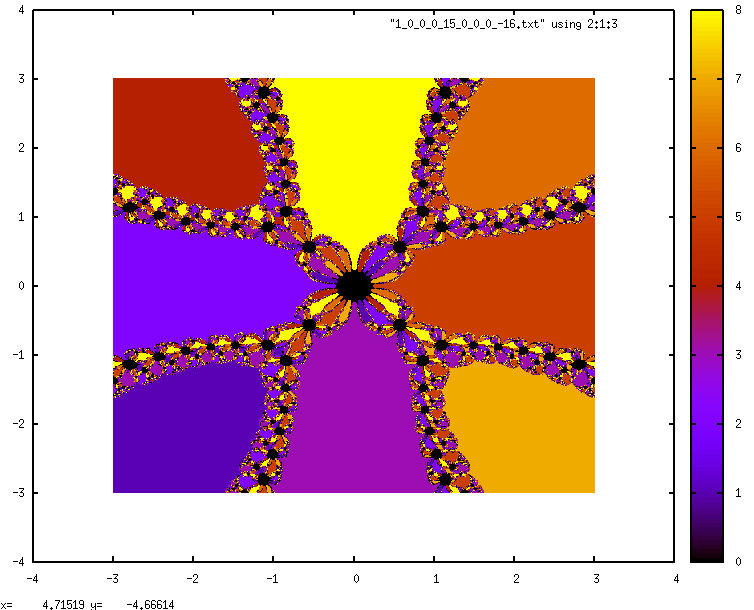
\includegraphics[scale=0.5]{1}
    \caption{Bacia de Convergência do polinômio P(x) = x$^8$ + 15x$^4$ -16}
    \vsp\vsp
    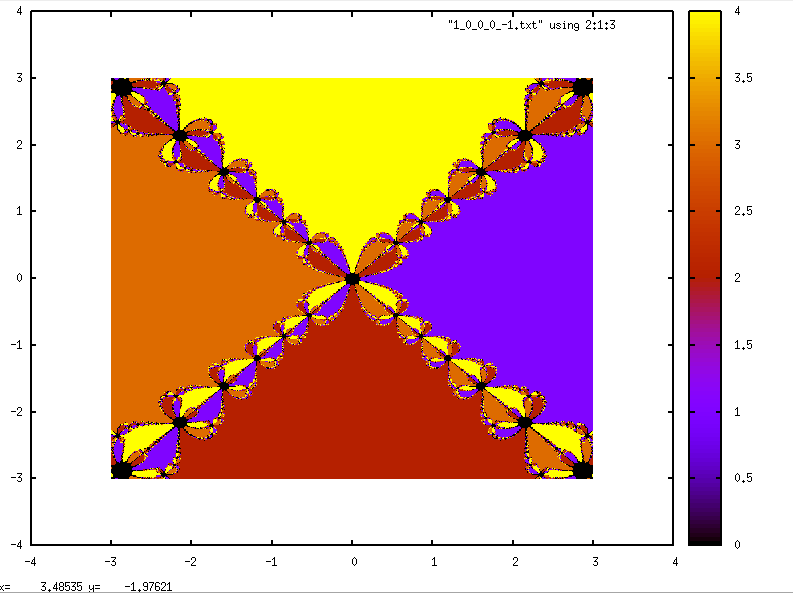
\includegraphics[scale=0.5]{2}
    \caption{Bacia de Convergência do polinômio P(x) = x$^4$ -1}
  \end{center}
\end{figure}

\begin{figure}[h!]
  \begin{center}
    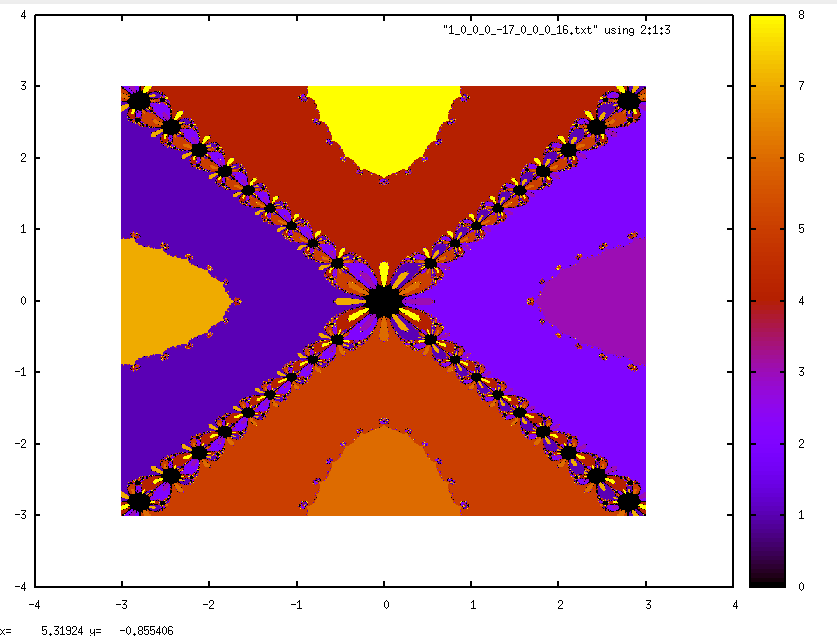
\includegraphics[scale=0.45]{3}
    \caption{Bacia de Convergência do polinômio P(x) = x$^8$ - 17x$^4$+16}
    \vsp\vsp
    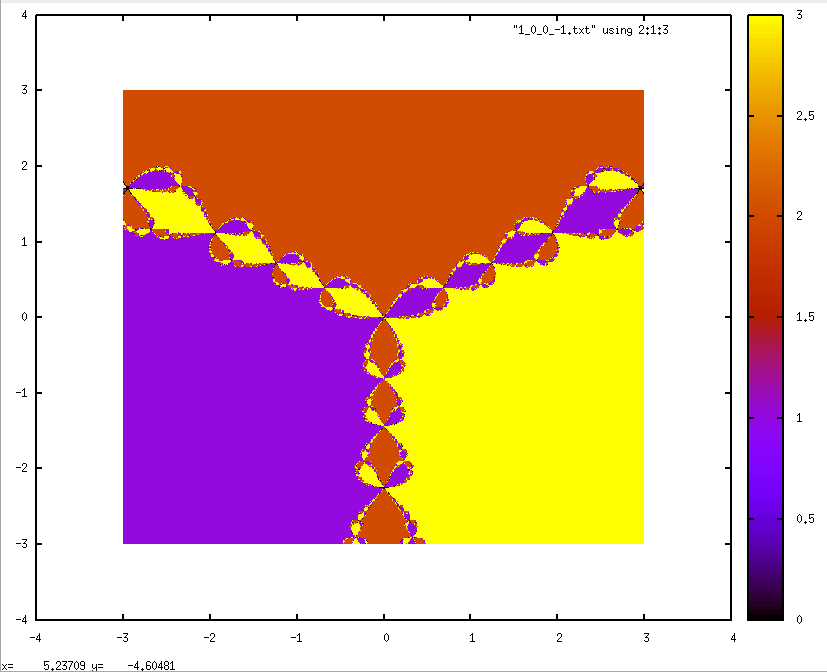
\includegraphics[scale=0.45]{4}
    \caption{Bacia de Convergência do polinômio P(x) = x$^3$ -1}
  \end{center}
\end{figure}

\begin{figure}[h!]
  \begin{center}
    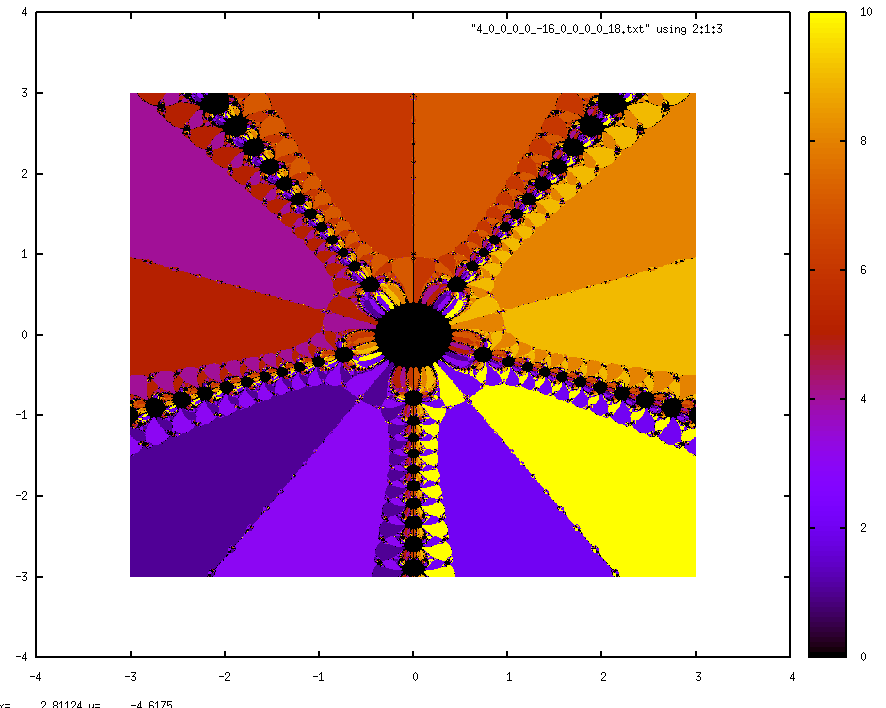
\includegraphics[scale=0.42]{5}
    \caption{Bacia de Convergência do polinômio P(x) = 4x$^{10}$ -16x$^5$ +18}
    \vsp\vsp
    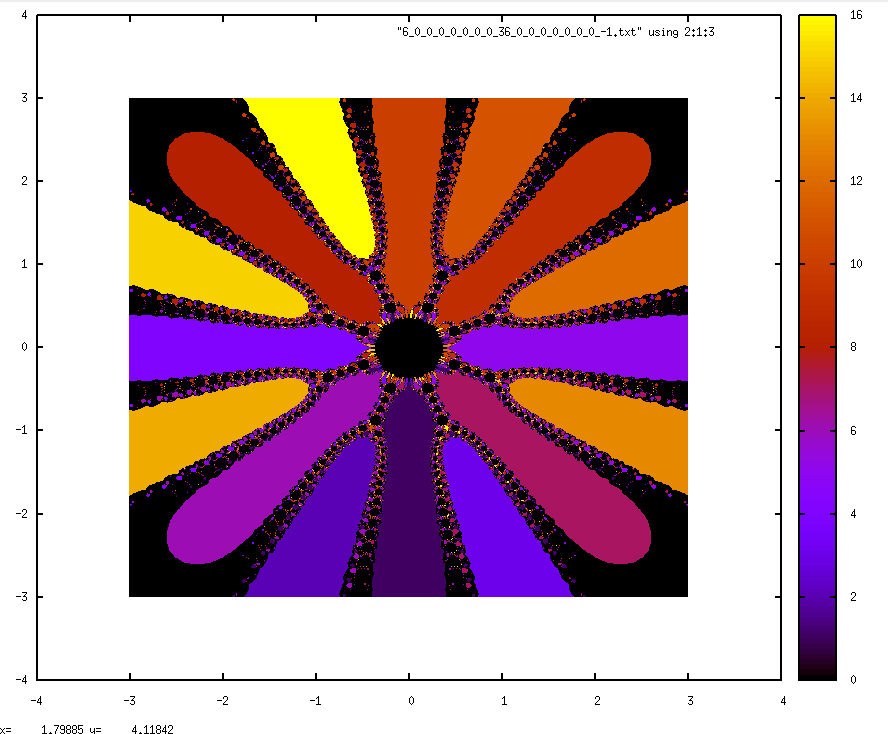
\includegraphics[scale=0.42]{6}
    \caption{Bacia de Convergência do polinômio P(x) = 6x$^{16}$ + 36x$^8$ -1}
  \end{center}
\end{figure}

\begin{figure}[h!]
  \begin{center}
    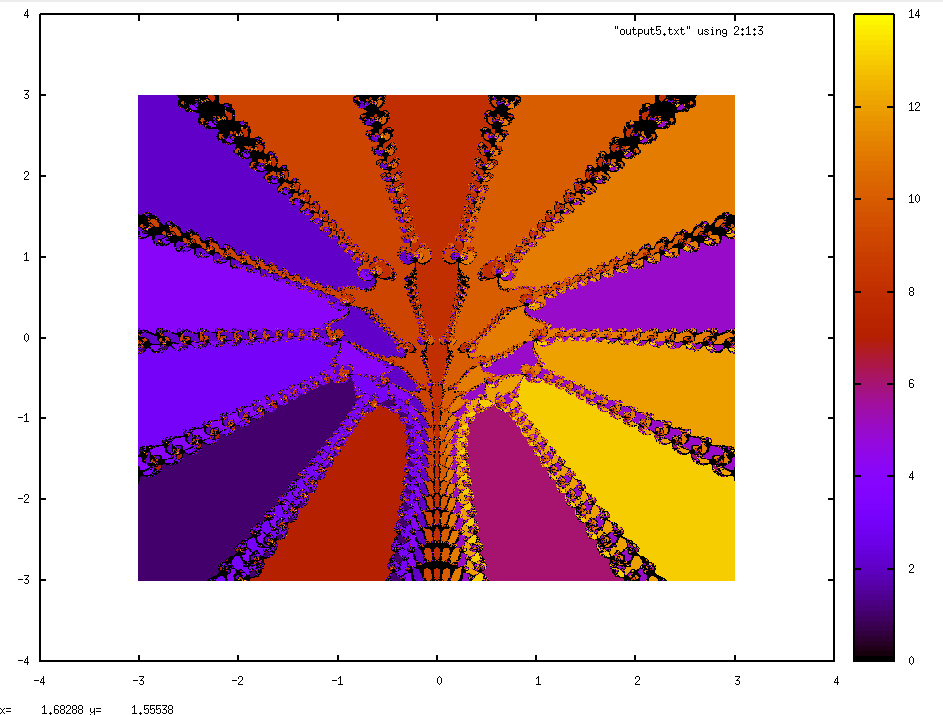
\includegraphics[scale=0.5]{7}
    \caption{Bacia de Convergência do polinômio P(x) = x$^{13}$ -2x$^{12}$ + 3x$^{11}$ -4x$^{10}$ + 5x$^9$ -6x$^8$ + 7x$^7$ -8x$^6$ + 9x$^5$ -10x$^4$ + 11x$^3$ -12x$^2$ + 13x -14}
  \end{center}
\end{figure}

\end{document}
